\documentclass[12pt,a4paper]{report}

% ==============================================================================
% ACADEMIC PROJECT REPORT TEMPLATE (VTU / ENGINEERING STANDARD)
% Parameterized college report template with institutional styling
% ==============================================================================

\usepackage[left=0.85in,right=0.85in,top=0.9in,bottom=0.9in]{geometry}
\usepackage{mathptmx} % Times New Roman font for text and math

% Set code elements and inline identifiers to document Times New Roman font
% (Prevents long identifiers/paths from overflowing right margins)
\renewcommand{\texttt}[1]{{\normalfont #1}}

\usepackage{setspace}
\onehalfspacing % 1.5 line spacing standard for university submissions
\setlength{\emergencystretch}{2em}

\usepackage{amsmath,amssymb,amsfonts}
\usepackage{booktabs,tabularx,multirow,longtable}
\usepackage{xcolor,colortbl}
\usepackage{listings}
\usepackage{fancyhdr}
\usepackage{caption}
\usepackage{subcaption}
\usepackage{hyperref}
\usepackage{titlesec}
\usepackage{graphicx}
\usepackage{enumitem}
\usepackage{tikz}
\usetikzlibrary{shapes.geometric, arrows.meta, positioning, calc, fit}

% ------------------------------------------------------------------------------
% Parameterized Metadata Configuration
% ------------------------------------------------------------------------------
\newcommand{\ProjectTitle}{Project Title Here}
\newcommand{\ProjectSubtitle}{Comprehensive Technical \& Experimental Report}
\newcommand{\CourseName}{Course Name and Code}
\newcommand{\BatchID}{Batch 2026\_XX\_01}
\newcommand{\InstitutionName}{KAMMAVARI SANGHAM INSTITUTE OF TECHNOLOGY}
\newcommand{\InstitutionShort}{K. S. Institute of Technology}
\newcommand{\InstitutionAffiliation}{(Affiliated to Visvesvaraya Technological University, Belagavi | Approved by AICTE, New Delhi)}
\newcommand{\DepartmentName}{Department of Computer Science \& Engineering}
\newcommand{\CityLocation}{Bengaluru -- 560109, Karnataka, India}
\newcommand{\AcademicYear}{2025--2026}

% ------------------------------------------------------------------------------
% Institutional Color Palette
% ------------------------------------------------------------------------------
\definecolor{primarybrand}{RGB}{128, 0, 0}    % Institutional Maroon
\definecolor{tableheader}{RGB}{240, 240, 240} % Neutral light gray
\definecolor{codebg}{RGB}{248, 249, 250}      % Light background for code
\definecolor{slateborder}{RGB}{100, 100, 100}

% List spacing configuration
\setlist{topsep=2pt,partopsep=0pt,parsep=0pt,itemsep=2pt}

% Hyperlink styling
\hypersetup{
    colorlinks=true,
    linkcolor=black,
    citecolor=black,
    urlcolor=blue!70!black,
    pdftitle={\ProjectTitle},
    pdfauthor={\BatchID}
}

% ------------------------------------------------------------------------------
% Header and Footer Formatting
% ------------------------------------------------------------------------------
\setlength{\headheight}{27pt}

\renewcommand{\headrule}{%
  \ifdim\headrulewidth>0pt\relax%
    \hbox to\headwidth{\color{primarybrand}\leaders\hrule height \headrulewidth\hfill}\vspace{2pt}%
  \fi%
}
\renewcommand{\footrule}{%
  \ifdim\footrulewidth>0pt\relax%
    \vspace{-4pt}\hbox to\headwidth{\color{primarybrand}\leaders\hrule height \footrulewidth\hfill}\vspace{4pt}%
  \fi%
}

% Standard body pages style (running maroon header and footer rules)
\fancypagestyle{fancy}{
    \fancyhf{}
    \fancyhead[L]{\textbf{\fontsize{10}{12}\selectfont \ProjectTitle}}
    \fancyfoot[L]{\fontsize{10}{12}\selectfont Dept. of CSE, \InstitutionShort}
    \fancyfoot[R]{\fontsize{10}{12}\selectfont Page \thepage}
    \renewcommand{\headrulewidth}{1.8pt}
    \renewcommand{\footrulewidth}{1.8pt}
}

% Preliminary pages style (Roman numerals, no header rule, no footer rule)
\fancypagestyle{preliminary}{
    \fancyhf{}
    \fancyfoot[C]{\fontsize{11}{13}\selectfont \thepage}
    \renewcommand{\headrulewidth}{0pt}
    \renewcommand{\footrulewidth}{0pt}
}

% Plain page style for chapter opening pages (includes running header and maroon rules)
\fancypagestyle{plain}{
    \fancyhf{}
    \fancyhead[L]{\textbf{\fontsize{10}{12}\selectfont \ProjectTitle}}
    \fancyfoot[L]{\fontsize{10}{12}\selectfont Dept. of CSE, \InstitutionShort}
    \fancyfoot[R]{\fontsize{10}{12}\selectfont Page \thepage}
    \renewcommand{\headrulewidth}{1.8pt}
    \renewcommand{\footrulewidth}{1.8pt}
}

% ------------------------------------------------------------------------------
% Chapter and Section Formatting
% ------------------------------------------------------------------------------
\titleformat{\chapter}[display]
  {\normalfont\bfseries\centering}
  {\fontsize{13}{15}\selectfont Chapter \thechapter}
  {0.2ex}
  {\fontsize{13}{15}\selectfont\MakeUppercase}
\titlespacing*{\chapter}{0pt}{-15pt}{15pt}

\titleformat{\section}
  {\normalfont\fontsize{11.5}{13.5}\bfseries}
  {\thesection}
  {0.8em}
  {}
\titlespacing*{\section}{0pt}{10pt}{4pt}

\titleformat{\subsection}
  {\normalfont\fontsize{10.5}{12.5}\bfseries}
  {\thesubsection}
  {0.8em}
  {}
\titlespacing*{\subsection}{0pt}{8pt}{3pt}

% Captions formatting
\captionsetup[figure]{font={small,it},labelfont={small,it},labelsep=colon,justification=centering}
\captionsetup[table]{font={small,bf},labelfont={small,bf},labelsep=colon,justification=centering,skip=6pt}

% TikZ Flowchart Styles
\tikzset{
    flowblock/.style = {rectangle, rounded corners, minimum width=3.2cm, minimum height=0.9cm, text centered, draw=black, fill=primarybrand!12, font=\fontsize{9.5}{11.5}\selectfont},
    processblock/.style = {rectangle, rounded corners, minimum width=3.4cm, minimum height=0.9cm, text centered, draw=black, fill=white, font=\fontsize{9}{11}\selectfont},
    decisionblock/.style = {diamond, aspect=2.2, minimum width=3cm, minimum height=1cm, text centered, draw=black, fill=white, font=\fontsize{9}{11}\selectfont},
    line/.style = {draw, -{Latex[length=2.5mm]}, thick}
}

\begin{document}

% ==============================================================================
% PRELIMINARY PAGES (ROMAN NUMERAL PAGINATION)
% ==============================================================================
\pagenumbering{roman}
\pagestyle{preliminary}

% ------------------------------------------------------------------------------
% TITLE PAGE
% ------------------------------------------------------------------------------
\begin{titlepage}
\begin{center}
    {\fontsize{15}{18}\bfseries \InstitutionName}\\[0.3em]
    {\fontsize{9.5}{12}\selectfont \InstitutionAffiliation}\\[0.5em]
    {\fontsize{11}{14}\bfseries \DepartmentName}\\[0.2em]
    {\fontsize{10}{13}\selectfont \CityLocation}\\[1.5em]

    {\color{primarybrand}\rule{\textwidth}{1.8pt}}\\[1.8em]

    {\fontsize{18}{22}\bfseries \ProjectTitle}\\[0.8em]
    {\fontsize{12}{15}\selectfont\textit{\ProjectSubtitle}}\\[1.2em]

    {\color{primarybrand}\rule{\textwidth}{1.8pt}}\\[2em]

    {\fontsize{11}{14}\selectfont Technical Report submitted in fulfillment of the academic requirements for:}\\[0.5em]
    {\fontsize{12}{15}\bfseries \CourseName}\\[0.3em]
    {\fontsize{11}{14}\bfseries Allocation / Batch: \BatchID}\\[2.5em]

    \begin{minipage}{0.48\textwidth}
        \begin{flushleft}
            \textbf{Submitted By:}\\[0.4em]
            \textbf{Student 1} (USN 1)\\[0.2em]
            \textbf{Student 2} (USN 2)\\[0.2em]
            \textbf{Student 3} (USN 3)\\[0.2em]
            \textbf{Student 4} (USN 4)
        \end{flushleft}
    \end{minipage}
    \hfill
    \begin{minipage}{0.48\textwidth}
        \begin{flushright}
            \textbf{Under the Guidance of:}\\[0.4em]
            \textbf{Prof. Faculty Guide}\\[0.2em]
            Assistant Professor\\[0.2em]
            \DepartmentName\\[0.2em]
            \InstitutionShort
        \end{flushright}
    \end{minipage}

    \vfill
    {\fontsize{11}{14}\selectfont Academic Year: \AcademicYear}
\end{center}
\end{titlepage}

\newpage

% ------------------------------------------------------------------------------
% ABSTRACT
% ------------------------------------------------------------------------------
\begin{center}
    {\fontsize{14}{16}\bfseries ABSTRACT}\\[1.5em]
\end{center}
\addcontentsline{toc}{chapter}{ABSTRACT}

Abstract paragraph summarizing project domain, problem statement, key system modules, algorithmic implementations, verification metrics, and syllabus Course Outcome (CO) mapping.

\newpage

% ------------------------------------------------------------------------------
% TABLE OF CONTENTS (GRID TABLE FORMAT)
% ------------------------------------------------------------------------------
\begin{center}
    {\fontsize{14}{16}\bfseries TABLE OF CONTENTS}\\[1.5em]
\end{center}

\begin{table}[h!]
\centering
\fontsize{10.5}{13.5}\selectfont
\begin{tabular}{|c|p{4.7in}|c|}
\hline
\rowcolor{tableheader}
\textbf{Chapter No.} & \multicolumn{1}{c|}{\textbf{Title}} & \textbf{Page No.} \\
\hline
& \textbf{ABSTRACT} & \textbf{ii} \\
\hline
\textbf{1.} & \textbf{INTRODUCTION AND OBJECTIVES} & \textbf{1} \\
& 1.1 Background and Problem Statement & 1 \\
& 1.2 Course Outcome Mapping and Objectives & 1 \\
\hline
\textbf{2.} & \textbf{THEORETICAL BACKGROUND} & \textbf{2} \\
& 2.1 Theoretical Foundations & 2 \\
\hline
\textbf{3.} & \textbf{SYSTEM REQUIREMENTS AND ARCHITECTURE} & \textbf{4} \\
& 3.1 Software and Hardware Specifications & 4 \\
& 3.2 Modular Repository Organization & 4 \\
\hline
\textbf{4.} & \textbf{ALGORITHMIC DESIGN AND METHODOLOGY} & \textbf{5} \\
& 4.1 Algorithmic Pseudocode and Core Implementations & 5 \\
& 4.2 Architectural Pipeline Flowcharts & 9 \\
\hline
\textbf{5.} & \textbf{IMPLEMENTATION AND RUNTIME DEMONSTRATION} & \textbf{13} \\
& 5.1 Source Code Architecture and Function Details & 13 \\
& 5.2 Runtime Execution Demonstrations and Verification Screenshots & 14 \\
& 5.3 Data Flow Pipeline Traces & 17 \\
\hline
\textbf{6.} & \textbf{TESTING METHODOLOGY AND VERIFICATION MATRIX} & \textbf{18} \\
& 6.1 Systematic Verification Strategy & 18 \\
& 6.2 Exhaustive Verification Matrix & 18 \\
\hline
\textbf{7.} & \textbf{SECURITY AND PERFORMANCE ANALYSIS} & \textbf{20} \\
& 7.1 Empirical Security and Complexity Analysis & 20 \\
& 7.2 Comparative Evaluation & 22 \\
\hline
\textbf{8.} & \textbf{APPLICATIONS AND CONCLUSION} & \textbf{23} \\
& 8.1 Real-World and Industrial Applications & 23 \\
& 8.2 Conclusion & 23 \\
\hline
& \textbf{REFERENCES} & \textbf{24} \\
\hline
& \textbf{GROUP CONTRIBUTION MATRIX} & \textbf{25} \\
\hline
& \textbf{PROJECT PRESENTATION PHOTOGRAPH} & \textbf{26} \\
\hline
\end{tabular}
\end{table}

\newpage

% ------------------------------------------------------------------------------
% LIST OF FIGURES (GRID TABLE FORMAT)
% ------------------------------------------------------------------------------
\begin{center}
    {\fontsize{14}{16}\bfseries LIST OF FIGURES}\\[1.5em]
\end{center}

\begin{table}[h!]
\centering
\fontsize{9.5}{12}\selectfont
\begin{tabular}{|c|p{4.8in}|c|}
\hline
\rowcolor{tableheader}
\textbf{Figure No.} & \multicolumn{1}{c|}{\textbf{Figure Title}} & \textbf{Page No.} \\
\hline
Fig 4.1 & Architectural Pipeline Flowchart & 9 \\
\hline
Fig 5.1 & Runtime Interface Demonstration & 14 \\
\hline
\end{tabular}
\end{table}

\vspace{1.5em}

% ------------------------------------------------------------------------------
% LIST OF TABLES (GRID TABLE FORMAT)
% ------------------------------------------------------------------------------
\begin{center}
    {\fontsize{14}{16}\bfseries LIST OF TABLES}\\[1.5em]
\end{center}

\begin{table}[h!]
\centering
\fontsize{9.5}{12}\selectfont
\begin{tabular}{|c|p{4.8in}|c|}
\hline
\rowcolor{tableheader}
\textbf{Table No.} & \multicolumn{1}{c|}{\textbf{Table Title}} & \textbf{Page No.} \\
\hline
Table 3.1 & Software Toolchain and Verified Dependencies & 4 \\
\hline
Table 6.1 & Complete Verification Matrix & 18 \\
\hline
Table 7.1 & Comparative Evaluation of Implemented Solutions & 22 \\
\hline
Table 8.1 & Group Contribution and Deliverable Ownership Matrix & 25 \\
\hline
\end{tabular}
\end{table}

\newpage

% ==============================================================================
% MAIN BODY CHAPTERS (ARABIC NUMERAL PAGINATION WITH RUNNING MAROON RULES)
% ==============================================================================
\pagenumbering{arabic}
\pagestyle{fancy}

% ------------------------------------------------------------------------------
% CHAPTER 1: INTRODUCTION AND OBJECTIVES
% ------------------------------------------------------------------------------
\chapter{Introduction and Objectives}

\section{Background and Problem Statement}
Detailed introduction, industry problem statement, and engineering scope.

\section{Course Outcome Mapping and Objectives}
Objectives, syllabus mapping, and educational outcomes.

\newpage

% ------------------------------------------------------------------------------
% CHAPTER 2: THEORETICAL BACKGROUND
% ------------------------------------------------------------------------------
\chapter{Theoretical Background}

\section{Theoretical Foundations}
Mathematical principles, algorithmic definitions, and literature background.

\newpage

% ------------------------------------------------------------------------------
% CHAPTER 3: SYSTEM REQUIREMENTS AND ARCHITECTURE
% ------------------------------------------------------------------------------
\chapter{System Requirements and Architecture}

\section{Software and Hardware Specifications}

\begin{table}[h!]
\centering
\fontsize{10}{13}\selectfont
\begin{tabular}{|l|l|p{3.2in}|}
\hline
\rowcolor{tableheader}
\textbf{Component} & \textbf{Environment / Tool} & \textbf{Purpose and Specification} \\
\hline
Operating System & Windows 11 / Linux & Primary execution and test environment \\
Runtime Language & Python 3.14 & Native implementation \\
Testing Tool & Pytest 8.x & Automated test harness \\
\hline
\end{tabular}
\caption{Software Toolchain and Verified Dependencies}
\end{table}

\section{Modular Repository Organization}
Architecture breakdown and directory structure.

\newpage

% ------------------------------------------------------------------------------
% CHAPTER 4: ALGORITHMIC DESIGN AND METHODOLOGY
% ------------------------------------------------------------------------------
\chapter{Algorithmic Design and Methodology}

\section{Algorithmic Pseudocode and Core Implementations}
% Dedicated page per core snippet:
Detailed explanation of algorithm logic with accompanying code snippet figure.

\newpage

\section{Architectural Pipeline Flowcharts}
% Dedicated page per flowchart:
Detailed explanation of pipeline sequence followed by centered native TikZ vector graphic.

\begin{figure}[h!]
\centering
\begin{tikzpicture}[node distance=1.1cm, auto]
    \node [flowblock] (start) {\textbf{Input Processing}};
    \node [processblock, below=0.6cm of start] (p1) {Process Step 1};
    \node [decisionblock, below=0.6cm of p1] (dec) {Condition Check?};
    \node [processblock, below=0.8cm of dec] (p2) {Final Output};
    
    \draw [line] (start) -- (p1);
    \draw [line] (p1) -- (dec);
    \draw [line] (dec) -- node [right, font=\scriptsize] {Yes} (p2);
    \draw [line] (dec.west) -- ++(-0.8cm,0) |- node [near start, left, font=\scriptsize] {No} (p1.west);
\end{tikzpicture}
\caption{System Execution Pipeline Flowchart}
\end{figure}

\newpage

% ------------------------------------------------------------------------------
% CHAPTER 5: IMPLEMENTATION AND RUNTIME DEMONSTRATION
% ------------------------------------------------------------------------------
\chapter{Implementation and Runtime Demonstration}

\section{Source Code Architecture and Function Details}
Module details and API interfaces.

\section{Runtime Execution Demonstrations}
CLI / GUI output evidence and screenshots.

\newpage

% ------------------------------------------------------------------------------
% CHAPTER 6: TESTING METHODOLOGY AND VERIFICATION MATRIX
% ------------------------------------------------------------------------------
\chapter{Testing Methodology and Verification Matrix}

\section{Systematic Verification Strategy}
Testing harness, Known-Answer Tests (KAT), and edge case validations.

\section{Exhaustive Verification Matrix}
Tabular presentation of verified test suite outcomes.

\newpage

% ------------------------------------------------------------------------------
% CHAPTER 7: SECURITY AND PERFORMANCE ANALYSIS
% ------------------------------------------------------------------------------
\chapter{Security and Performance Analysis}

\section{Empirical Security and Complexity Analysis}
Mathematical cryptanalysis, complexity analysis, and empirical benchmarks.

\section{Comparative Evaluation}
Benchmarking implemented modules against industry baselines.

\newpage

% ------------------------------------------------------------------------------
% CHAPTER 8: APPLICATIONS AND CONCLUSION
% ------------------------------------------------------------------------------
\chapter{Applications and Conclusion}

\section{Real-World and Industrial Applications}
Practical deployments and real-world relevance.

\section{Conclusion}
Summary of achievements and future scope.

\newpage

% ------------------------------------------------------------------------------
% REFERENCES
% ------------------------------------------------------------------------------
\begin{center}
    {\fontsize{14}{16}\bfseries REFERENCES}\\[1.5em]
\end{center}
\addcontentsline{toc}{chapter}{REFERENCES}

\begin{enumerate}[label={[\arabic*]}, leftmargin=2em, itemsep=6pt]
    \item Standard or Textbook Reference (e.g. Stallings, W. (2017). Cryptography and Network Security).
    \item RFC or NIST Publication Reference.
\end{enumerate}

\newpage

% ------------------------------------------------------------------------------
% GROUP CONTRIBUTION MATRIX
% ------------------------------------------------------------------------------
\begin{center}
    {\fontsize{14}{16}\bfseries GROUP CONTRIBUTION MATRIX}\\[1.5em]
\end{center}
\addcontentsline{toc}{chapter}{GROUP CONTRIBUTION MATRIX}

\begin{table}[h!]
\centering
\fontsize{10}{13}\selectfont
\begin{tabular}{|l|l|p{3.2in}|}
\hline
\rowcolor{tableheader}
\textbf{Student Name} & \textbf{USN} & \textbf{Module / Deliverable Responsibilities} \\
\hline
Student 1 & 1KS... & Core Algorithm Implementation \& Test Suite \\
Student 2 & 1KS... & Architectural Design \& Pipeline Flowcharts \\
Student 3 & 1KS... & Runtime Interface \& Verification Traces \\
Student 4 & 1KS... & Empirical Benchmarking \& Technical Documentation \\
\hline
\end{tabular}
\caption{Group Contribution and Deliverable Ownership Matrix}
\end{table}

\newpage

% ------------------------------------------------------------------------------
% PROJECT PRESENTATION PHOTOGRAPH
% ------------------------------------------------------------------------------
\begin{center}
    {\fontsize{14}{16}\bfseries PROJECT PRESENTATION PHOTOGRAPH}\\[1.5em]
\end{center}
\addcontentsline{toc}{chapter}{PROJECT PRESENTATION PHOTOGRAPH}

\vspace{1.5em}

\begin{figure}[h!]
\centering
\includegraphics[width=0.88\textwidth]{figures/team_presentation.jpg}
\vspace{0.8em}
\caption{Official Project Presentation and Technical Defense -- \BatchID}
\end{figure}

\end{document}
